\chapter{NIST Special Publication 800-90B}
\label{chap:NIST800-90B}
\section{General}

Topic of this thesis is an analysis of a Linux Random Number Generator's outcome delivered to kernel consumers, as introduced in \ref{sub:get-rnd-int-long}. Verification and estimation of entropy is 
a very difficult task, since there is no explicit definition for randomness. Hence, for a series of values generated by an RNG, randomness i.e. a sufficient degree of entropy is admitted, if the absence of any discernible pattern within a generated record can be diagnosed.
To assess the outcome and reliability of random number generating devices or implementations, several frameworks have been published, providing recommendations regarding the solid construction and validation of PRNG and TRNG sources. These also encompass a set of statistical tests and guidance how to conduct a profound verification (see \cite{robert2006dieharder, rukhin2010nist, turan2018nist}).
The National Institute of Standards and Technology (NIST) publishes a series of documents that describe U.S. federal government computer security policies, procedures and guidelines called NIST 800 series (see \cite[]{nist800pub}). To implement the analysis of this thesis, two Special Publications on the subject of validation and assessment of entropy and random number generation has been chosen:

\begin{table}[H]
	\centering
	\label{tab:nist800sps}
	\begin{tabular}{lll}\\ \hline 
		Number & Title & Release Date \\ \hline \hline 
		800-90B & \makecell[l]{Recommendation for the Entropy Sources Used for\\Random Bit Generation} & 1/10/2018 \\ \hline 
		800-22 Rev. 1a & \makecell[l]{A Statistical Test Suite for Random and Pseudorandom\\Number Generators for Cryptographic Applications} & 4/30/2010 \\ \hline 
	\end{tabular}
	\caption{Applied NIST Special Publications of the 800 Series (Status Final)}
\end{table} 


For this analysis, a framework based on 'Recommendation for the Entropy Sources Used for Random Bit Generation, NIST Special Publication 800- 90B' \cite{turan2018nist} has been chosen, able to deliver
usable guidance that will give conservative estimates on the amount of entropy in an entropy
source \cite{turan2015random}. The final version of the framework has been published in january 2018 and thus is very up to date. Beside that this decision has been met, since not just the outcome of and RNG can be assessed but also it's input. As mentioned in \ref{sec:int-rnd}, the Linux RNG executed on a Xen virtualized machine is not able to obtain noise from most designated sources. In fact, interrupt noise is the only input delivered during the initialization phase. Hence, to achieve a comprehensive analysis, an assessment of this input is considered to be required.\\
'NIST Special Publication (SP) 800-90' (a series consisting of three documents) specifies how to design an test 

 is all about
generating random numbers for cryptography. In SP 800-90, this is a two-stage process: first, an
entropy source provides an impossible-to-guess seed. Then, a deterministic cryptographic
algorithm (called a DRBG--deterministic random bit generator--in SP 800-90) expands the seed
into a long sequence of values that may be safely used for keys, IVs, nonces, etc.
\cite{turan2015random}.



 When assessing entropy by the second part of the series, 'NIST Special Publication 800-90B' (in the following referred to as NSP800-90B), an estimation can be achieved via 
two different tracks. Depending on an assumption regarding an entropy source, which has to be substantiated, the IID i.e. the Non-IID track should be used to analyze assumed random input 
\cite{turan2018nist}. The outcome of an analysis is an estimation of entropy, ascertained by statistical tests expressed in \textit{bits of entropy}. In the following sections, an introduction to these procedures, required to comprehend the results in TODO[Evaludation] is given.



%-----------------------------------------------
%NIST Special Publication (SP) 800-90 (a series consisting of three documents) is all about
%generating random numbers for cryptography. In SP 800-90, this is a two-stage process: first, an
%entropy source provides an impossible-to-guess seed. Then, a deterministic cryptographic
%algorithm (called a DRBG--deterministic random bit generator--in SP 800-90) expands the seed
%into a long sequence of values that may be safely used for keys, IVs, nonces, etc.
%\cite{turan2015random}

\section{Definitions \& Terminology}

\subsection{Distinction: Noise / Entropy / Randomness / RNG}
In literature, terms describing the in- and output of RNGs are sometimes used in a generic and partially confusing manner. For this thesis, the following terminology will be used, intending to distinguish regarding the maturity, source and purpose of (pseudo) random numbers.

\begin{itemize}
	\item \textbf{Entropy} Entropy is a property of a variable or value describing its certain degree of unpredictability. 
	\item \textbf{Noise} Noise is the input passed to an RNG or the state of an intermediate processing stage.
	While there might be a wide range in maturity, in general, noise is not assumed to provide a cryptographic safe degree of entropy. Since the Linux RNG enriches entropy via various steps (see \ref{fig:linux-prng-arch}) depending on the stage \textit{Noise} will be subdivided into:
	\begin{itemize}
		\item \textbf{Raw Noise} \textit{Noise} sources of the Linux RNG, delivering external physical states like interrupts (see \ref{sec:inp-src-lprng}).
		\item \textbf{Pre-processed Noise} Raw Noise being pre-processed via the fast-pool, assumed to have a poor level of \textit{Entropy} (see \ref{sub:fast-pool}).
		\item \textbf{Conditioned Noise} \textit{Noise} prepared by a conditioning component and hence providing an advanced level of \textit{Entropy}, like the input-pool (see \ref{sub:input-pool}).	
	\end{itemize}
	\item \textbf{Randomness} The outcome of an RNG delivered to a user mode or kernel consumer. This output is assumed to provide a cryptographic safe degree of \textit{Entropy}.
	\item \textbf{Entropy Source} The generic term for any kind of sources dedicated to deliver values assumed to provide a certain degree of \textit{Entropy}. This includes all kind of \textit{Noise Sources} as well as \textit{Random Sources}.	
	\item \textbf{RBG/RNG} NIST 800 uses the more generalizing term \textit{RBG (Random Bit Generator)} instead of \textit{RNG (Random Number Generator)}. Since this thesis relates to Linux x86 Kernel where random numbers are always obtained and applied on at least byte level, the term \textit{RNG} will be used.
\end{itemize}

\subsection{The formal Definition of Entropy}
In Information theory, for a set of information units, entropy in generall describes the level of disorder i.e. the unpredictability of each single unit's state at a given alphabet. Various formal definitions of entropy exist \cite{hagerty2012entropy}, while the definition of Shannon (see \ref{fig:form-entropy-shan}) is quite common for a binary alphabet. 

\begin{figure}[H]
	\begin{align*}
	\displaystyle H(X) := \sum_{s \in {0,1}} I(p_s) p_s = \sum_{s \in {0,1}} -\lg_2 \frac{1}{p_s} p_s && \text{$p_s$ = P(X=s)}
	\end{align*}
	\caption{Formal definiton of entropy by Shannon for a binary alphabet}
	\label{fig:form-entropy-shan}
\end{figure}
According to Shannon, entropy is defined as the product of self-information \textit{I} multiplied by the expected value. For a binary alphabet, it can be measured in unit \textit{bits}. 



\section{NIST Special Publication 800-90 B}

The NIST Special Publication (SP) 800-90 series of recommendations provides 
guidance on the validation and construction of Pseudo- and Non-deterministic Random Number Generators that can be used for cryptographic secure applications. More precisely, the recommendation specifies how to design and validate noise delivering sources that are used as input for RNGs. Transfered to the Linux RNG this verification approach can be applied to the raw sources described in \ref{sec:inp-src-lprng} as well as on conditioned or pre-processed noise of the input- i.e. fast-pool (\ref{sub:input-pool}, \ref{sub:fast-pool}). The series consist of three parts. NSP800-90A and NSP800-90C refer to the construction of RNG mechanisms, while NSP800-90B addresses the analysis and validation of sources delivering noise. A source that conforms to this recommendation can be used by RNGs to produce a sequence of random values \cite{rukhin2010nist} i.e. randomness.\\
The validation process described by NSP800-90B consist of several sequential and iterative steps. For each step, a number of prerequisites and assumption is defined. A step can be a task required to prepare the next step or a test procedure consisting of several statistical test. In general, the validation process is all about determining entropy estimates, which are the outcome of particular test procedures applied on recorded noise datasets. Traditional statistical procedures like applied by NSP800-22 would fail, since this frameworf is testing under the hypothesis of unbiased, independent distributed values. The statistical test procedures of NSP800-90B are aware that noise sources will most likely not deliver entropy at a high level and hence assess accordingly. Figure \ref{fig-entropy-est-strategy} gives a overview of the entire Entropy Estimation Strategy of NSP800-90B. The following sections will explain relevant components of this strategy more detailed.

 \begin{figure}[H]
 	\centering
 	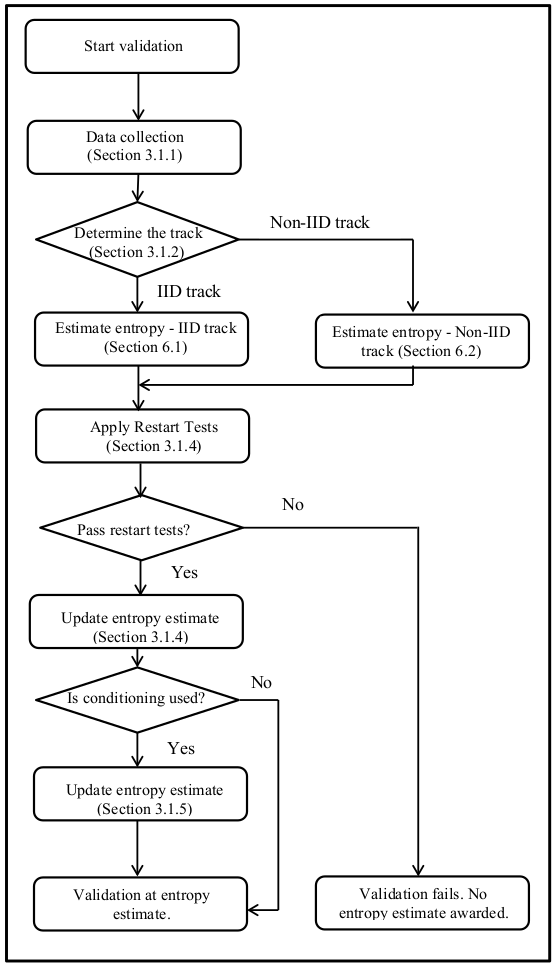
\includegraphics[scale=0.6]{img/nsp800-90b-entropy-est-strategy.png}
 	\caption{Entropy Estimation Strategy according to NIST SP 800-90B (from \cite{turan2018nist}, references illustrated refer to the publication)}
 	\label{fig-entropy-est-strategy}
 \end{figure}

\subsection{Min-Entropy}\label{sub:min-entropy}
In NSP800-90B, statistical test are bundled to test procedures. Each single test within a procedure delivers two related values, $p_{max}$ and min-entropy. The min-entropy of an independent discrete random variable $X$
that takes values from the set $A$ with probability $p_i$ is defined as $H$.

\begin{equation}
A = \{x_1, x_2, x_3, ..., x_k\}
\label{eq:min-ent-A}
\end{equation}
\begin{equation}
Pr(X=x_i) = p_i 
\Domain{i=\{1,...,k\}}
\end{equation}
\begin{equation}
H = \underset{1\leq i\leq k}{\mathrm{min}}(-\log_2p_i) = -\log_2 \underset{1\leq i\leq k}{\mathrm{max}}p_i
\end{equation}

If $X$ has min-entropy $H$, then the probability $p_{max}$ of observing any particular value for $X$ is $\le$ $2^{-H}$ \cite{turan2018nist}. The outcome of a test procedure is a single min-entropy value, representing the lowest min-entropy delivered by a specific statistical test.

\subsection{Data Records}\label{sub:data-records}
The test procedures of NSP800-90B are applied on data sets resulting from recording sequential produced values from the noise sources to be analyzed. A data record should at least provide 1.000.000 samples directly obtained from the source. If this number can not be achieved, which is the case for the interrupt noise source analyzed in this thesis, several smaller sets may be concatenated, while each set shall contain at least 1000 samples. In total the data record shall finally contain 1.000.000 samples \cite{turan2018nist}. A downstream test procedure, required to be conducted for a comprehensive result is the \textit{restart test}. This procedure requires to record the value sequences delivered by a noise source 1000 times. For each restart, 1000 samples shall be tracked. The recorded data is merged to a single binary data file, the restart matrix. 
NSP800-90B does not require i.e. recommend to pass the recorded (merged) data directly to the test procedures. After recording values from a noise source, data may be vetted. If it is obvious, also by the nature of a an analyzed noise source, that there might be a variation in a fixed pattern regarding the obtained values, those may be trimmed at a fix pattern. Though it is essential that the sequence is kept, i.e. the trimmed values are aligned in the same order as delivered by the noise source. The standard requires to document and advocate this approach, since the analysis result is reduced to those bytes. If a noise source f.e. delivers four byte values based on simple incrementation, it is obvious that the higher bytes of each value in the sequence will have less variation than the lower ones. In this case, trimming is recommended.

\subsection{IID vs. Non-IID Track}\label{sub:iid-noniid-track}
\ref{fig-entropy-est-strategy}
 sdfsdf
 \gls{python}
Independent and identically distributed random variables
% the lowest  

%  \ref{sub:min-entropy}

% taking into account the
% expected statistical 
%
%the noise source will not produce unbiased, independent binary data
%
%NIST SP 800-22
%
%Since, in most cases,
%the noise source will not produce unbiased, independent binary data, traditional statistical
%procedures (e.g., the randomness tests described in NIST SP 800-22) that test the hypothesis of
%unbiased, independent bits will almost always fail, and thus are not useful for monitoring the noise
%source. In general, tests on the noise source need to be tailored carefully, taking into account the
%expected statistical behavior of the correctly operating noise source.












